\chapter{Valutazione dei risultati}
\label{chap:results-evaluation}

L'unione delle necessità di comunicazione di rete ed il coinvolgimento di sistemi
embedded nel contributo di questa tesi rende la validazione dei risultati difficile
da automatizzare in maniera efficace.
Per ridurre i tempi di sviluppo è stato quindi adottato un approccio più manuale:
sono stati creati dei programmi specifici che utilizzano i vari componenti
implementati coprendo diversi casi e piattaforme, per poi verificare manualmente
che il risultato sia quello atteso.

\section{Il wrapper Zenoh pico: test del ping-pong}
\label{sec:zenoh-pico-ping-pong-test}

Il test del ping-pong consiste nel far comunicare due nodi in un ciclo infinito:
ad ogni iterazione il nodo attende di ricevere un nuovo valore sul topic opposto,
lo modifica a piacere e lo pubblica sul suo topic dedicato, dove l'altro nodo sarà
in attesa con una logica analoga.
Per evitare situazioni di \emph{deadlock} nella comunicazione, la partenza sarà
assimmetrica, con un nodo che inizia inviando il valore e l'altro in attesa di
ricevere (\Cref{fig:ping-pong-sequence}).

\begin{figure}[H]
    \centering
    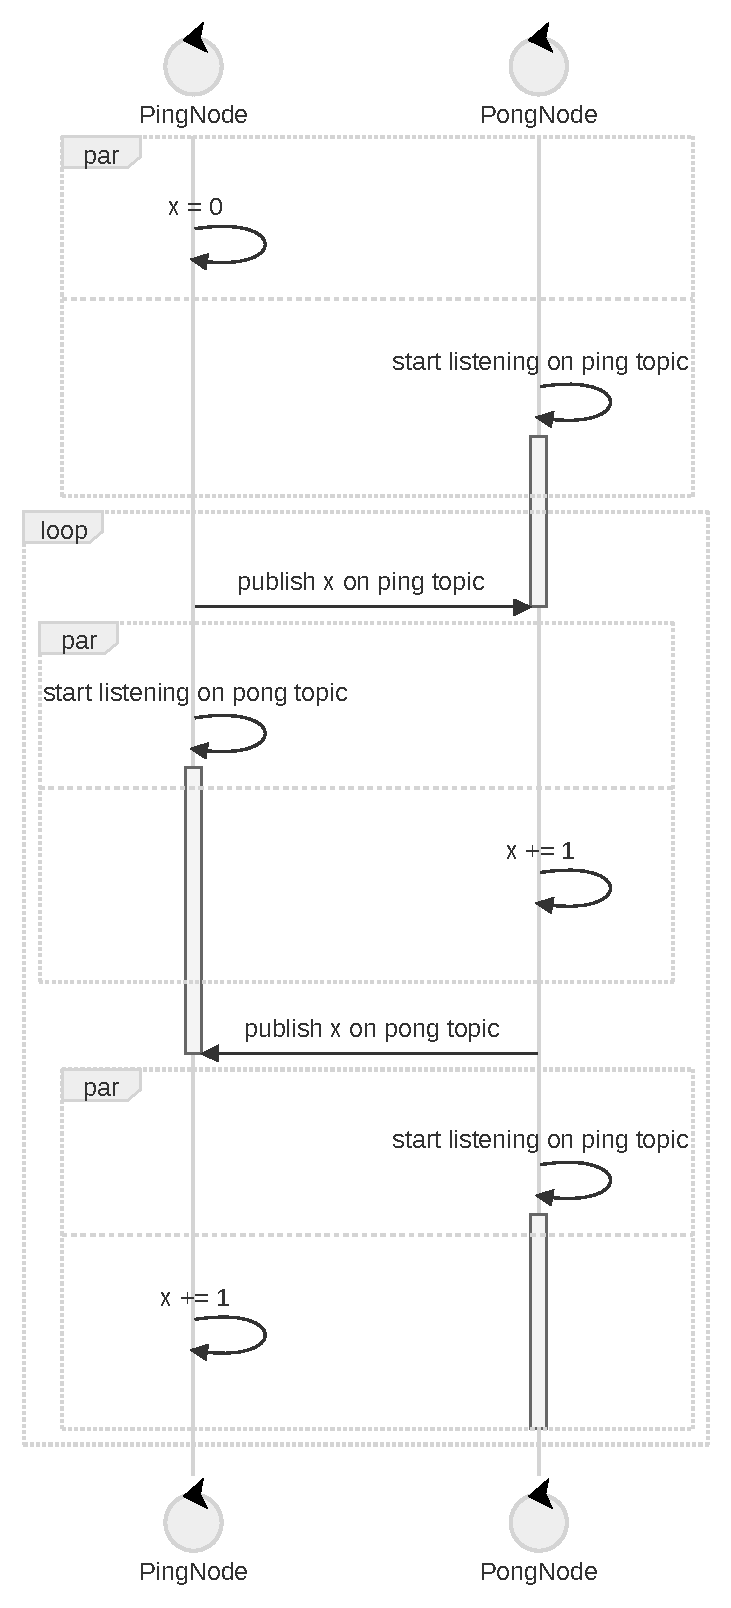
\includegraphics[height=0.9\dimexpr\textheight\relax]{figures/ping-pong-sequence}
    \caption{Diagramma di sequenza del test del ping-pong.}
    \label{fig:ping-pong-sequence}
\end{figure}

\subsection{Obbiettivi}
\label{ssec:ping-pong-objectives}

Questo test non utilizza nè \ac{YAAIR} nè la rete per esso creata, bensì ha
lo scopo di verificare il corretto funzionamento del wrapper per Zenoh pico implementato
nella \cref{sec:zenoh-pico-wrapper} anche al di fuori
del contesto di un programma aggregato.

\subsection{Implementationze}
\label{ssec:ping-pong-implementation}

Essendo un test per il wrapper di Zenoh pico, è stato pensato per i sistemi
embedded che andranno poi ad utilizzare questa implementazione del protocollo
all'interno della rete per \ac{YAAIR}.
Sono quindi previsti programmi distinti, eseguibili su dispositivi separati,
rappresentanti i due diversi nodi descritti nella \cref{sec:zenoh-pico-ping-pong-test}.

Dopo una fase di inizializzazione per avviare la sessione Zenoh e dichiarare i
\emph{publisher} e \emph{subscriber} necessari, il nodo \texttt{ping} imposta
un valore \texttt{x=0}, mentre il nodo \texttt{pong} si mette in ascolto per nuovi
messaggi sul topic \texttt{ping/value} sfruttando la \ac{API} asincrona del wrapper
definita nella \cref{sec:closure-system}.
A questo punto inizia il ciclo infinito di scambio del valore (\Cref{lst:ping-pong-test}):

\begin{enumerate}
    \item il nodo \texttt{ping} pubblica il valore di \texttt{x} sul topic
    \texttt{ping/value}, e si mette in ascolto sul topic analogo \texttt{pong/value}.
    \item il nodo \texttt{pong}, che era già in ascolto per nuovi valori sul topic
    \texttt{ping/value}, riceve il valore di \texttt{x}, lo incrementa e lo pubblica
    nuovamente sul topic \texttt{pong/value}.
    \item Analogamente, il nodo \texttt{ping} riceve il nuovo valore aggiornato,
    lo incrementa a sua volta e ricomincia il ciclo infinito fino a quando non viene
    interrotto il programma manualmente.
\end{enumerate}

\lstinputlisting[
    language=Rust,
    caption={Implementazione del test del ping-pong per il wrapper di Zenoh pico.},
    label={lst:ping-pong-test}
]{listings/ping-pong-test.rs}

\subsection{Risultati}
\label{ssec:ping-pong-results}

Il test è stato eseguito su due ESP32-C3 Mini 1, dispositivi della famiglia Espressif
dotati di un processore con architettura RiscV a 32 bit e di moduli per la
connettività tramite WiFi.
Ognuno di questi dispositivi esegue un solo programma tra \texttt{ping}
e \texttt{pong}, caricato via cavo dalla macchina host.

Possiamo notare dai log mostrati in \cref{fig:ping-pong-logs} che il valore viene
trasferito tra un nodo e l'altro, di conseguenza la comunicazione \emph{pub/sub}
tramite il wrapper Zenoh pico funziona correttamente.

\begin{figure}[H]
    \centering
    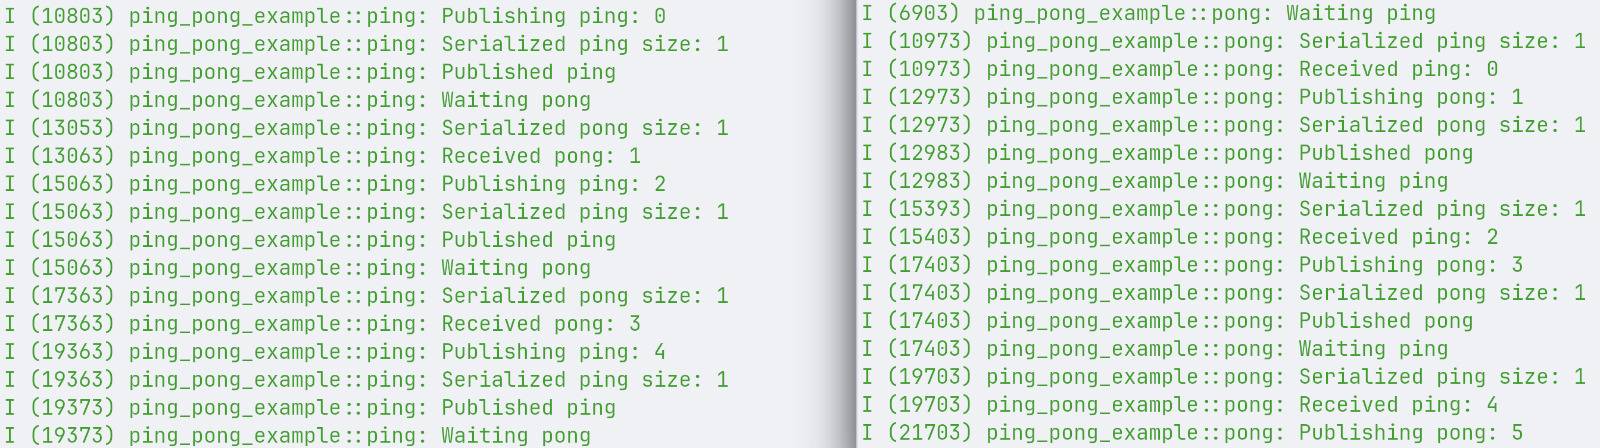
\includegraphics[width=1\linewidth]{figures/ping-pong-logs}
    \caption[Log di esecuzione del test del ping pong.]{
    Log di esecuzione del test del ping pong. È possibile vedere come ogni volta
    che viene scambiato il valore, viene incrementato di 1 prima di essere rimandato
    indietro. Inoltre, a puro scopo informativo, viene anche mostrata la dimensione
    della sequenza di byte rappresentante il valore.}
    \label{fig:ping-pong-logs}
\end{figure}

\section{La rete Zenoh: test del gradiente}
\label{sec:zenoh-network-gradient-test}

Descrizione del test del gradiente e la sua struttura.

\subsection{Obbiettivi}
\label{ssec:gradient-objectives}

Obbiettivi del test del gradiente.

\subsection{Setup}
\label{ssec:gradient-setup}

Setup del test del gradiente: numero di esp utilizzati, tipo, tipo di rete
(wifi o cablata), etc\dots

\subsection{Risultati}
\label{ssec:gradient-results}

Risultati del test del gradiente.
